\chapter{Umelá inteligencia a jej vývin}
Umelá inteligencia ako pojem v počítačovej vede bol prvý krát predstavený na konferencií Darthmouth v roku 1956 Johnom McCarthym\cite{Corduck}. Na tejto istej konferencií debutoval prvý program, ktorý využíval automatizované uvažovanie, "Logic Theorist". Tento program bol schopný dokázať 38 z 52 matematických teorémou z knihy \textit{Principia Mathematica}. Jeden z dôkazov bol dokonca považovaný za elegantnejší než ručne vypočítaný originál z knihy. Táto konferencia sa taktiež považuje za "narodenie" umelej inteligencie ako vedy.\\Logic Theorist predstavil niekoľko konceptov ktoré sa stali kľúčovými pre výskum umelej inteligencie:\\\textbf{Vyhľadávací strom}\\
\begin{wrapfigure}{r}{0.50\textwidth}
    \centering
    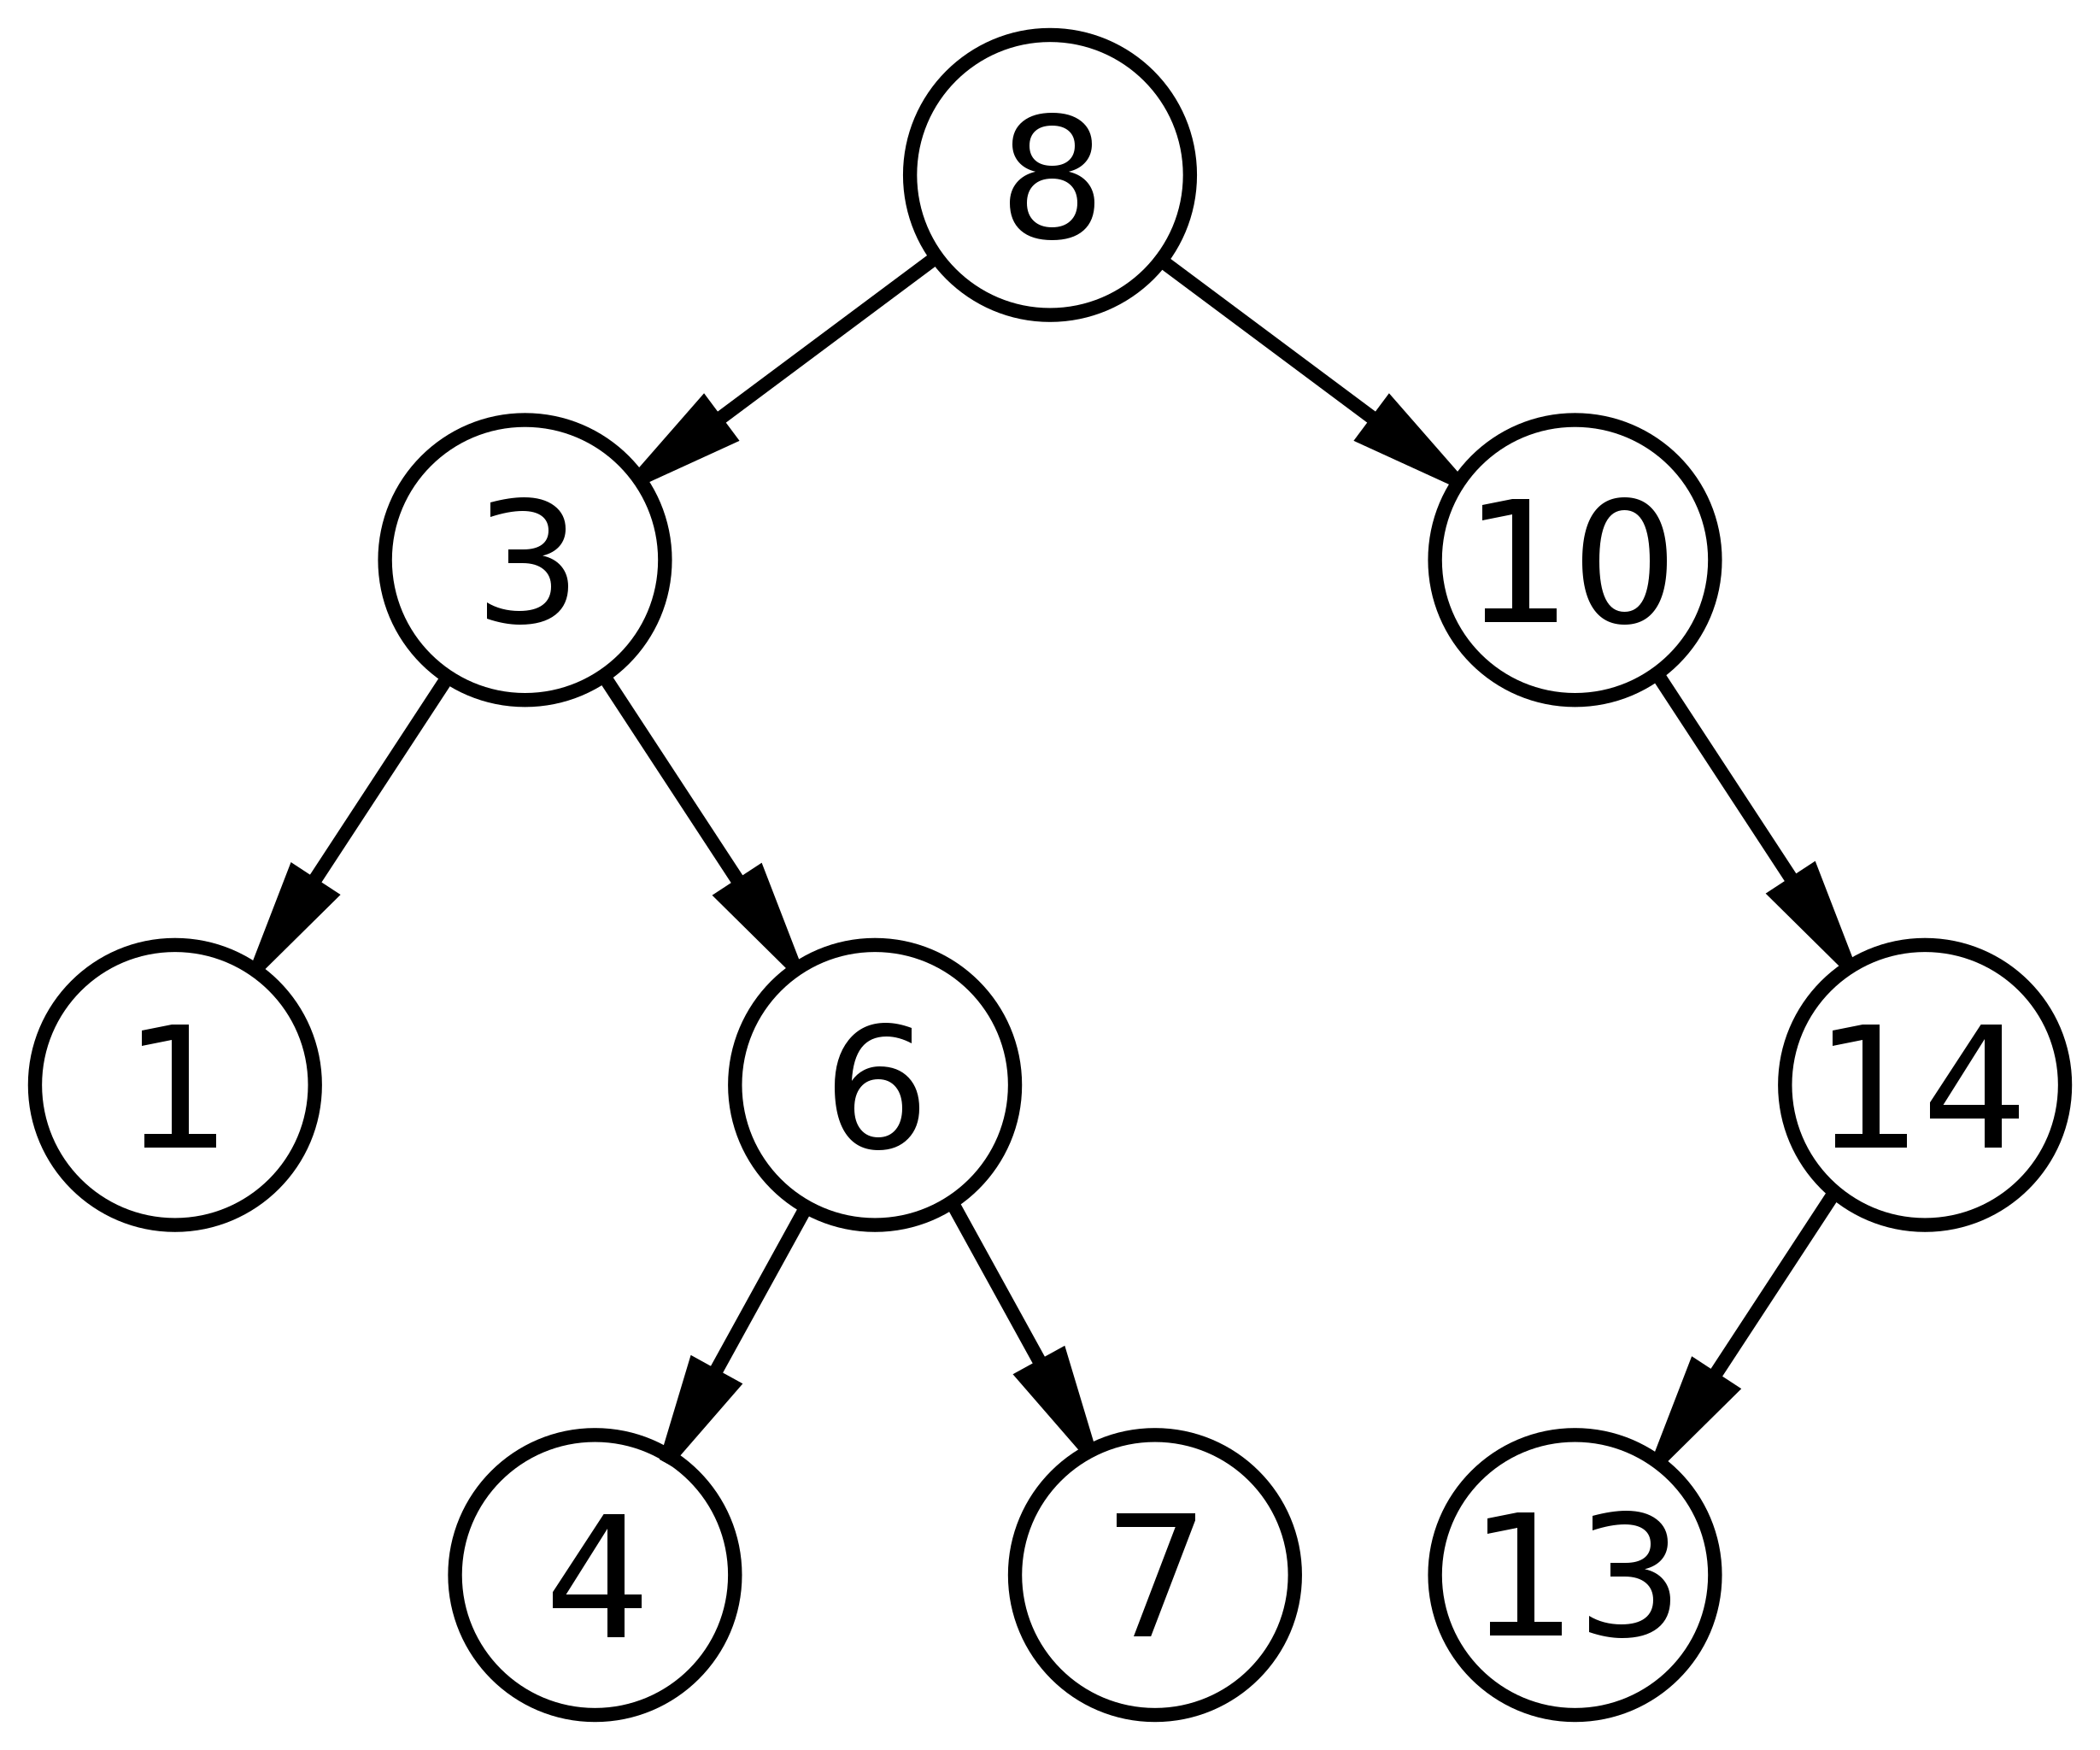
\includegraphics[width=0.25\textwidth]{BinarySearchTree}
\end{wrapfigure}Logic Theorist prechádzal cez binárny vyhľadávací strom. Koreňom stromu bola počiatočná hypotéza a každá vetva bola dedukcia založená na pravidlách logiky. Cieľom programu bolo dostať sa k výroku, ktorý sa snažil dokázať. Všetky kroky, cez ktoré program prešiel tvoria dôkaz – sériu tvrdení, ktoré viedli od hypotézy k výroku, ktorý mal dokázať.\\\textbf{Heuristika}  